\section{Méthodologie}
\label{sec:methodologie}

\subsection{Workflow proposé}
\label{sec:workflow}

La figure~\ref{fig:workflow} résume la démarche suivie, de l'archive téléchargée jusqu'aux analyses finales. Deux choix structurent l'ensemble. D'abord, le jeu de données est audité et nettoyé \emph{avant} tout découpage, de sorte qu'aucune image (ni sa copie) ne puisse se retrouver à la fois dans l'apprentissage et dans le test. Ensuite, l'ensemble de test est isolé une fois pour toutes : il ne sert ni à choisir les hyperparamètres ni à sélectionner les modèles. Tout le travail d'ajustement se fait par validation croisée sur la partie restante, que nous appelons \og ensemble de développement \fg{}.

\begin{figure}[htbp]
\centering
\begin{tikzpicture}[
  node distance=0.55cm and 0.42cm,
  box/.style={draw=accent, fill=lightaccent!55, rounded corners=3pt, align=center, font=\footnotesize, minimum height=1.75cm, text width=3.15cm, inner sep=3pt},
  data/.style={box, fill=softgray, draw=inkgray},
  key/.style={box, fill=accent, draw=accent, text=white},
  arrow/.style={-{Stealth[length=2.3mm]}, thick, draw=inkgray}
]
\node[data] (raw) {\textbf{Données brutes}\\ Kaggle / Mendeley\\ 2\,521 images, 5 classes};
\node[box, right=of raw] (clean) {\textbf{Audit et nettoyage}\\ intégrité, doublons exacts (MD5), quasi-doublons};
\node[box, right=of clean] (split) {\textbf{Découpage stratifié}\\ test : 15\,\% à l'écart\\ développement : 85\,\% en 5 plis};
\node[box, right=of split] (prep) {\textbf{Prétraitement}\\ $256\times256 \rightarrow 224\times224$\\ normalisation};
\node[box, below=of prep] (aug) {\textbf{Augmentation}\\ en ligne, sur GPU,\\ apprentissage seulement};
\node[key, left=of aug] (train) {\textbf{Entraînement}\\ 4 backbones $\times$\\ \{FE, PFT, FFT\}\\ + CNN from scratch};
\node[box, left=of train] (cv) {\textbf{Validation croisée}\\ 5 plis : choix de l'époque sur le pli de validation};
\node[box, left=of cv] (fusion) {\textbf{Fusion}\\ concaténation d'embeddings (15 combinaisons), vote souple};
\node[data, below=0.55cm of $(cv.south)!0.5!(train.south)$, text width=12.4cm, minimum height=1.05cm] (eval) {\textbf{Évaluation sur l'ensemble de test} : accuracy, précision, rappel, F1, matrices de confusion, courbes ROC et AUC, robustesse aux dégradations, coût de calcul, interprétation par Grad-CAM};
\draw[arrow] (raw) -- (clean);
\draw[arrow] (clean) -- (split);
\draw[arrow] (split) -- (prep);
\draw[arrow] (prep) -- (aug);
\draw[arrow] (aug) -- (train);
\draw[arrow] (train) -- (cv);
\draw[arrow] (cv) -- (fusion);
\draw[arrow] (fusion.south) -- (fusion.south |- eval.north);
\draw[arrow] (cv.south) -- (cv.south |- eval.north);
\draw[arrow] (train.south) -- (train.south |- eval.north);
\draw[arrow, dashed] (split.north) -- ++(0,0.35) -| ($(prep.east)+(0.4,0)$) |- (eval.east) node[pos=0.25, right, font=\scriptsize, text=inkgray] {test};
\end{tikzpicture}
\caption{Workflow général du projet. L'ensemble de test (flèche pointillée) n'intervient qu'à l'étape finale d'évaluation.}
\label{fig:workflow}
\end{figure}

\subsection{Description du jeu de données}
\label{sec:dataset}

\subsubsection{Origine et contenu}

Nous utilisons le \emph{Sugarcane Leaf Disease Dataset} publié par Daphal et Koli sur Mendeley Data \cite{daphal2022sugarcane} sous licence CC~BY~4.0, dans la copie mise en ligne sur Kaggle par N. Sankalana \cite{sankalana2024sugarcane} et proposée dans l'énoncé du projet. Nous avons vérifié, fichier par fichier, que la copie Kaggle est identique à l'archive d'origine (mêmes noms, mêmes tailles). D'après l'article qui l'accompagne \cite{daphal2023enhancing}, les photographies ont été prises en août et septembre, entre 9~h et 17~h et par temps clair, dans plusieurs exploitations de Nagargaon (district de Pune, Maharashtra, Inde), avec trois smartphones d'entrée de gamme (deux modèles Vivo et un POCO M2 Pro). Les prises de vue ont été réalisées au champ, avec l'arrière-plan naturel (sol, autres feuilles, débris), et l'étiquetage a été confié à des agents agricoles et à des agriculteurs expérimentés.

L'archive contient \textbf{2\,521 images JPEG} réparties en \textbf{cinq classes} : une classe saine et quatre maladies (figure~\ref{fig:samples}). La description officielle annonce 2\,569 images, mais l'archive n'en contient que 2\,521 ; l'écart porte presque entièrement sur la classe Mosaic (511 annoncées, 462 présentes). Les symptômes, tels que décrits dans la littérature phytopathologique \cite{rott2000guide, viswanathan2011sugarcane}, se distinguent ainsi :
\begin{itemize}
  \item \textbf{Healthy} (feuille saine) : limbe vert et homogène, nervure centrale blanchâtre intacte ;
  \item \textbf{Mosaic} (mosaïque, d'origine virale) : alternance de plages vert clair et vert foncé, sous forme de stries ou de marbrures parallèles aux nervures \cite{viswanathan2005mosaic} ;
  \item \textbf{RedRot} (pourriture rouge, due au champignon \emph{Colletotrichum falcatum}) : lésions allongées rouge vif le long de la nervure centrale, dont le centre s'éclaircit avec le temps \cite{viswanathan2021redrot} ;
  \item \textbf{Rust} (rouille brune ou orangée) : petites pustules allongées brun-orangé, alignées le long des nervures \cite{hoy2009brownrust, zhao2011orangerust} ;
  \item \textbf{Yellow} (maladie de la feuille jaune, due au virus ScYLV) : jaunissement qui part de la nervure centrale et gagne progressivement le limbe \cite{rassaby2003yellow, elsayed2015scylv}.
\end{itemize}

\begin{figure}[htbp]
\centering
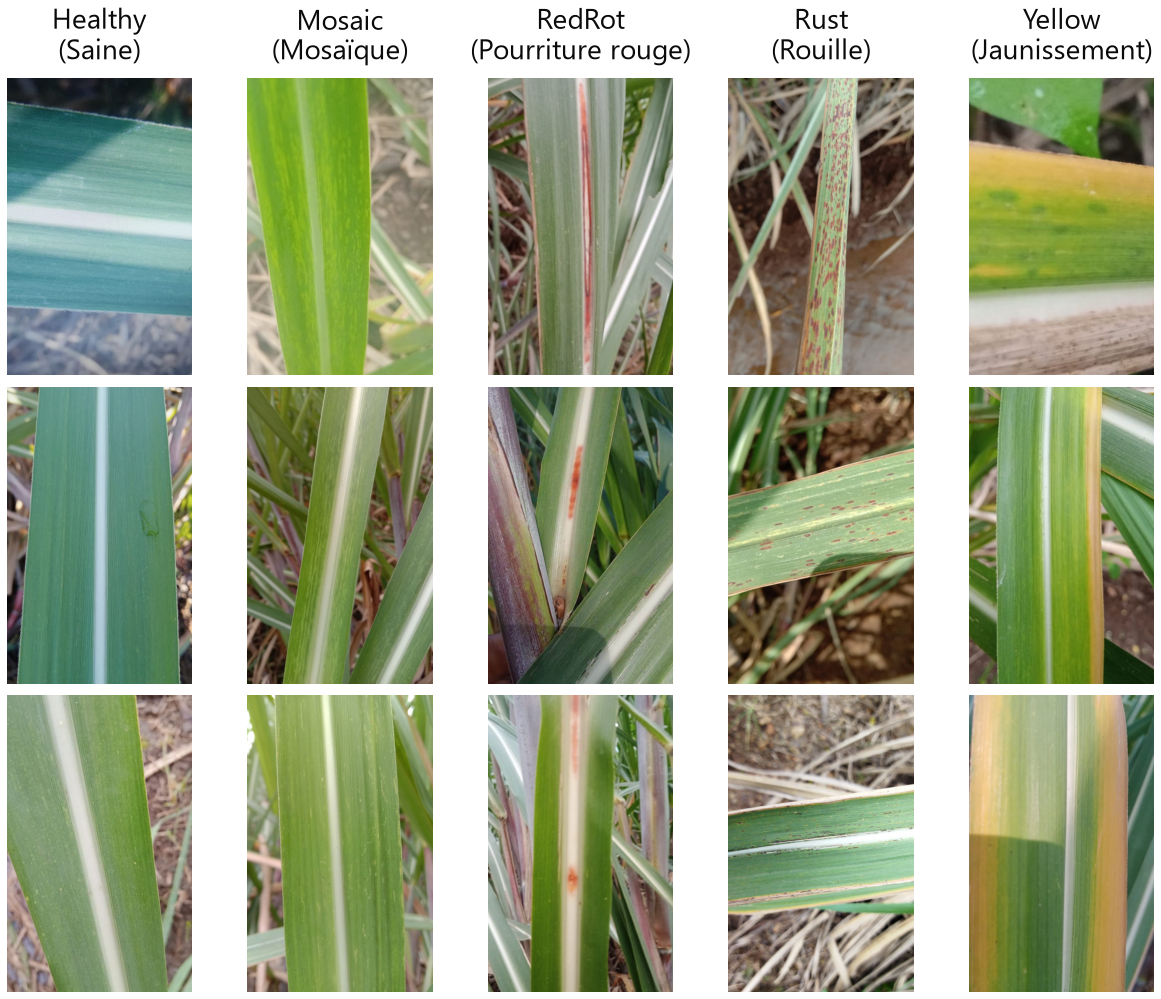
\includegraphics[width=0.92\textwidth]{dataset_samples.png}
\caption{Exemples d'images tirées au hasard pour chacune des cinq classes (recadrage d'affichage uniquement).}
\label{fig:samples}
\end{figure}

Les images ne sont ni uniformes ni normalisées : nous avons recensé 119 résolutions différentes, de $240\times292$ à $1600\times1600$ pixels. Deux formats portrait dominent, $493\times1040$ (958 images) et $780\times1040$ (580 images), ce qui donne un rapport largeur/hauteur médian de 0,56 (figure~\ref{fig:sizes}). Toutes les images sont en couleurs (RVB) et aucune n'est corrompue.

\begin{figure}[htbp]
\centering
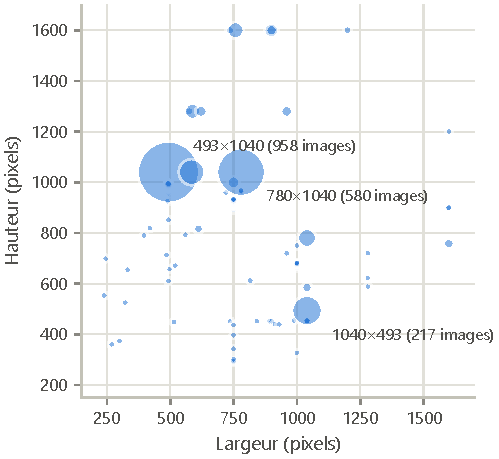
\includegraphics[width=0.52\textwidth]{image_sizes.pdf}
\caption{Résolutions des images brutes. La surface de chaque disque est proportionnelle au nombre d'images ayant cette résolution.}
\label{fig:sizes}
\end{figure}

\subsubsection{Audit et nettoyage}

Avant d'entraîner quoi que ce soit, nous avons calculé l'empreinte MD5 de chaque fichier. Le résultat a été une vraie surprise : \textbf{210 images sont des copies exactes} d'autres images (184 groupes de doublons). Elles se concentrent dans trois classes : 86 copies pour Mosaic (soit 18,6\,\% de la classe), 67 pour Rust et 46 pour Healthy. Aucun doublon ne relie deux classes différentes, il ne s'agit donc pas d'erreurs d'étiquetage. Le danger est ailleurs : avec un découpage aléatoire, une image et sa copie peuvent tomber l'une dans l'apprentissage, l'autre dans le test, et le modèle est alors évalué sur des images qu'il a déjà vues. Aucun des articles que nous avons consultés et qui utilisent ce jeu de données ne mentionne ce problème.

Nous avons ensuite cherché les quasi-doublons, c'est-à-dire la même photographie légèrement recadrée ou ré-encodée. Chaque image est réduite à une vignette $32\times32$ en niveaux de gris, centrée et réduite, puis comparée à toutes les autres par corrélation. Au-delà d'une corrélation de 0,90, toutes les paires examinées visuellement correspondaient à la même scène, prise deux fois ou recadrée de quelques pixels, et toujours dans la même classe ; en dessous de 0,85 apparaissaient au contraire des paires de feuilles différentes, simplement semblables par leur composition. Nous avons donc retenu le seuil de 0,90 et conservé une seule image par groupe, ce qui retire 24 images supplémentaires. Le jeu final compte \textbf{2\,287 images} (figure~\ref{fig:cleaning} et tableau~\ref{tab:dataset}).

\begin{figure}[htbp]
\centering
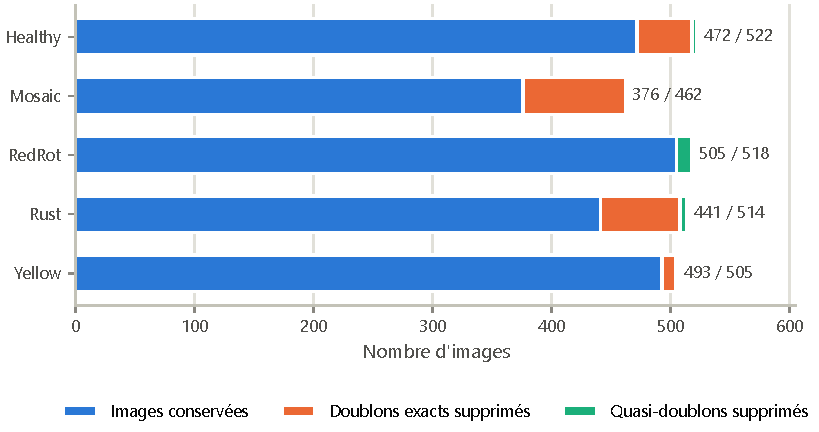
\includegraphics[width=0.8\textwidth]{class_distribution.pdf}
\caption{Effet du nettoyage sur chaque classe : images conservées et images supprimées (doublons exacts et quasi-doublons). Les nombres indiquent les images conservées sur le total initial.}
\label{fig:cleaning}
\end{figure}

\subsubsection{Répartition apprentissage, validation et test}

Le découpage est stratifié, afin que chaque sous-ensemble conserve les proportions des classes. On isole d'abord \textbf{15\,\% des images pour le test} (344 images), qui ne seront utilisées qu'une seule fois, à la fin. Les 1\,943 images restantes sont réparties en \textbf{cinq plis stratifiés} : à tour de rôle, chaque pli sert à la validation (environ 389 images) pendant que les quatre autres servent à l'apprentissage (environ 1\,554 images). Chaque modèle est donc entraîné cinq fois, ce qui donne une répartition d'environ 68\,\% pour l'apprentissage, 17\,\% pour la validation et 15\,\% pour le test. Le tableau~\ref{tab:dataset} détaille les effectifs ; les autres plis ne diffèrent du premier que d'une image au plus par classe.

\begin{table}[htbp]
\centering
\caption{Effectifs par classe avant et après nettoyage, et répartition pour le premier pli de la validation croisée.}
\label{tab:dataset}
\begin{tabular}{llrrrrr}
\toprule
\textbf{Classe} & \textbf{Nom français} & \textbf{Brut} & \textbf{Nettoyé} & \textbf{Apprentissage} & \textbf{Validation} & \textbf{Test} \\
\midrule
\tableinput{tables/dataset_table.tex}
\bottomrule
\end{tabular}
\end{table}

Après nettoyage, le jeu reste à peu près équilibré : la classe la plus petite (Mosaic, 376 images) représente 74\,\% de la plus grande (RedRot, 505 images). Ce léger déséquilibre ne justifie pas de pondérer la fonction de perte, mais il explique que nous rapportions des métriques moyennées par classe (moyenne \emph{macro}) en plus de l'accuracy.

\subsection{Prétraitement}
\label{sec:pretraitement}

Le prétraitement a deux rôles. Il met d'abord toutes les images au format que les réseaux attendent : une taille fixe et des valeurs d'intensité comparables à celles vues pendant le pré-entraînement. Il conditionne aussi la qualité de l'optimisation, car des entrées centrées et réduites stabilisent la descente de gradient et accélèrent la convergence \cite{ioffe2015batch}. Dans le cas des maladies des plantes, Barbedo rappelle que la variabilité des conditions d'acquisition (éclairage, cadrage, résolution) est l'une des principales sources d'erreur des systèmes automatiques \cite{barbedo2016review} ; un prétraitement uniforme limite au moins la part de cette variabilité qui ne relève pas des symptômes.

\paragraph{Redimensionnement.} Les images sont redimensionnées une fois pour toutes en $256\times256$ pixels (interpolation de Lanczos), puis ramenées à $224\times224$ à l'entrée du réseau, résolution à laquelle les quatre modèles pré-entraînés ont été conçus ou évalués. Ce redimensionnement ne conserve pas les proportions : une image portrait de $493\times1040$ est étirée horizontalement. Nous l'avons préféré à un recadrage central, qui aurait supprimé jusqu'à la moitié de la feuille, alors que les lésions (de pourriture rouge en particulier) se trouvent souvent vers les extrémités. La déformation est la même à l'apprentissage et au test, et les réseaux s'y adaptent sans difficulté. La version $256\times256$ est stockée sur disque au format PNG, sans perte, ce qui évite de redécoder les JPEG d'origine à chaque époque.

\paragraph{Normalisation.} Les intensités sont d'abord ramenées dans $[0,1]$, puis chaque canal $c$ est centré et réduit :
\begin{equation}
\tilde{x}_c = \frac{x_c - \mu_c}{\sigma_c}, \qquad c \in \{R, V, B\}.
\label{eq:norm}
\end{equation}
Pour les modèles pré-entraînés, nous reprenons les statistiques utilisées lors de leur pré-entraînement, faute de quoi les filtres appris recevraient des entrées décalées : $\mu=(0{,}485 ; 0{,}456 ; 0{,}406)$ et $\sigma=(0{,}229 ; 0{,}224 ; 0{,}225)$ pour MobileNetV4, ConvNeXtV2 et SE-ResNet-50, et $\mu=\sigma=(0{,}5 ; 0{,}5 ; 0{,}5)$ pour les poids d'EfficientNetV2 issus de l'implémentation TensorFlow d'origine. Pour le CNN entraîné from scratch, nous utilisons les statistiques de notre propre jeu, calculées sur l'ensemble de développement uniquement : $\mu=(0{,}499 ; 0{,}530 ; 0{,}382)$ et $\sigma=(0{,}193 ; 0{,}193 ; 0{,}199)$. Le canal bleu, nettement plus faible, reflète la dominante verte des images. Dans le code, cette normalisation est la première couche de chaque modèle : tous les modèles reçoivent ainsi exactement les mêmes images, ce qui simplifie aussi l'évaluation de la robustesse et les visualisations Grad-CAM.

\subsection{Augmentation de données}
\label{sec:augmentation}

Avec environ 1\,550 images d'apprentissage par pli, un réseau de plusieurs millions de paramètres finit par mémoriser les exemples. L'augmentation de données consiste à générer, à chaque époque, des variantes plausibles des images d'apprentissage, de façon à enseigner au modèle les invariances attendues (position, orientation, éclairage) sans collecter de nouvelles données \cite{shorten2019survey, perez2017effectiveness}. Elle agit comme un régulariseur et compte parmi les moyens les plus efficaces de limiter le surapprentissage sur de petits jeux de données.

Les transformations ont été choisies pour rester réalistes. Une feuille photographiée au champ peut apparaître à n'importe quelle position et dans n'importe quel sens, d'où le recadrage aléatoire, les symétries et une légère rotation. L'éclairage varie au cours de la journée, d'où les variations de luminosité et de contraste. En revanche, nous n'avons volontairement pas modifié la teinte et seulement très peu la saturation : la couleur est ici un symptôme (le jaune de la classe Yellow, le rouge de la classe RedRot), et la perturber reviendrait à brouiller l'information que le modèle doit apprendre. Concrètement, pour chaque image d'un lot, on tire indépendamment :
\begin{itemize}
  \item un recadrage aléatoire couvrant une fraction $a \sim \mathcal{U}(0{,}6 ; 1)$ de la surface, de rapport d'aspect $r$ tel que $\log r \sim \mathcal{U}(\log\tfrac{3}{4}, \log\tfrac{4}{3})$, placé au hasard dans l'image ;
  \item une rotation d'angle $\alpha \sim \mathcal{U}(-15^\circ, 15^\circ)$ ;
  \item une symétrie horizontale et une symétrie verticale, chacune avec une probabilité de 0,5 ;
  \item des facteurs de luminosité et de contraste dans $[0{,}75 ; 1{,}25]$ et un facteur de saturation dans $[0{,}85 ; 1{,}15]$.
\end{itemize}

Plutôt que d'enchaîner plusieurs opérations sur le processeur, les quatre transformations géométriques sont combinées en une seule transformation affine, appliquée sur GPU à tout le lot à la fois. Pour une image, les coordonnées normalisées $(u', v')$ du pixel de sortie sont envoyées vers les coordonnées $(u, v)$ de l'image source par
\begin{equation}
\begin{pmatrix} u \\ v \end{pmatrix} =
\begin{pmatrix} f_x\, s_x \cos\alpha & -f_y\, s_y \sin\alpha \\ f_x\, s_x \sin\alpha & f_y\, s_y \cos\alpha \end{pmatrix}
\begin{pmatrix} u' \\ v' \end{pmatrix} +
\begin{pmatrix} t_x \\ t_y \end{pmatrix},
\label{eq:affine}
\end{equation}
avec $s_x = \sqrt{a\,r}$ et $s_y=\sqrt{a/r}$ (tailles relatives du recadrage), $f_x, f_y \in \{-1, 1\}$ (symétries) et $t_x \sim (1-s_x)\,\mathcal{U}(-1,1)$, $t_y \sim (1-s_y)\,\mathcal{U}(-1,1)$ (position du recadrage). L'image est ensuite rééchantillonnée par interpolation bilinéaire ; les zones qui sortent de l'image source après rotation sont remplies par réflexion plutôt qu'en noir. Les modifications photométriques suivent, image par image, avec $g$ la luminance du pixel et $\bar{g}$ sa moyenne sur l'image :
\begin{equation}
x \leftarrow b\,x, \qquad x \leftarrow \bar{g} + c\,(x-\bar{g}), \qquad x \leftarrow g + s\,(x-g),
\label{eq:photo}
\end{equation}
chaque étape étant suivie d'un écrêtage dans $[0,1]$. L'augmentation n'est appliquée qu'aux images d'apprentissage ; les images de validation et de test sont seulement redimensionnées. Enfin, pour un pli donné, tous les modèles reçoivent les mêmes lots, dans le même ordre et avec les mêmes tirages aléatoires, puisque les générateurs sont initialisés avec la même graine. La figure~\ref{fig:augmentation} montre quelques variantes obtenues.

Ce choix d'implémentation a aussi une raison pratique. Sous Windows, les processus auxiliaires du chargeur de données de PyTorch démarrent lentement (chacun recharge toute la bibliothèque) et, au-delà de quelques-uns, leur démarrage échouait faute de mémoire virtuelle, ce qui bloquait l'entraînement. Garder les 2\,287 images en mémoire (environ 450~Mo) et faire l'augmentation sur GPU a supprimé le problème tout en accélérant les époques.

\begin{figure}[htbp]
\centering
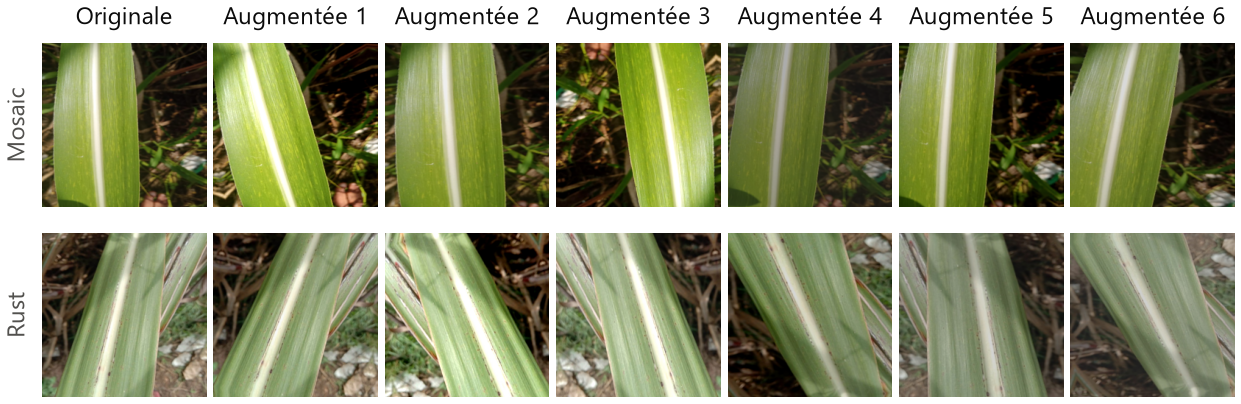
\includegraphics[width=\textwidth]{augmentation_examples.png}
\caption{Image d'origine et six variantes produites par l'augmentation, pour une feuille atteinte de mosaïque et une feuille atteinte de rouille.}
\label{fig:augmentation}
\end{figure}

\subsection{Modèles utilisés}
\label{sec:modeles}

\subsubsection{Architectures pré-entraînées}

Les quatre familles imposées par l'énoncé sont représentées par une variante de taille comparable, disponible avec des poids ImageNet-1k dans la bibliothèque \texttt{timm} \cite{wightman2019timm}.

\paragraph{EfficientNetV2-S \cite{tan2021efficientnetv2}.} EfficientNet \cite{tan2019efficientnet} a popularisé la mise à l'échelle conjointe de la profondeur, de la largeur et de la résolution d'un réseau de base obtenu par recherche d'architecture. La version~2 remplace, dans les premiers étages, les blocs MBConv (convolution en profondeur et module Squeeze-and-Excitation) par des blocs Fused-MBConv, où une convolution $3\times3$ classique se substitue à la paire expansion--convolution en profondeur, nettement plus rapide sur GPU. Elle a été conçue pour accélérer l'entraînement, avec une recherche d'architecture tenant compte du temps d'apprentissage et un apprentissage progressif où la taille des images et la régularisation augmentent au fil des époques ; les auteurs annoncent un entraînement jusqu'à quatre fois plus rapide que les modèles antérieurs, pour un nombre de paramètres jusqu'à 6,8 fois plus faible. Nous utilisons la variante S (\texttt{tf\_efficientnetv2\_s.in1k}).

\paragraph{MobileNetV4-Conv-M \cite{qin2024mobilenetv4}.} MobileNetV4 est la dernière génération de la famille MobileNet \cite{howard2019searching}, pensée pour les téléphones et les accélérateurs embarqués. Son bloc de base, l'\emph{Universal Inverted Bottleneck} (UIB), généralise le bloc inversé de MobileNetV2 en rendant optionnelles deux convolutions en profondeur, ce qui permet à la recherche d'architecture de choisir, étage par étage, le compromis le plus efficace pour le matériel visé. Nous utilisons la variante convolutive moyenne (\texttt{mobilenetv4\_conv\_medium.e500\_r224\_in1k}), la plus légère des quatre.

\paragraph{ConvNeXtV2-T \cite{woo2023convnextv2}.} ConvNeXt \cite{liu2022convnet} a montré qu'un réseau purement convolutif, modernisé avec des recettes issues des Vision Transformers (convolutions en profondeur $7\times7$, LayerNorm, activation GELU, goulot d'étranglement inversé), pouvait rivaliser avec eux. ConvNeXtV2 ajoute une couche de \emph{Global Response Normalization} (GRN), qui renforce la compétition entre canaux, et un pré-entraînement auto-supervisé par masquage (FCMAE) suivi d'un fine-tuning supervisé. Nous utilisons la variante Tiny (\texttt{convnextv2\_tiny.fcmae\_ft\_in1k}).

\paragraph{SE-ResNet-50 \cite{hu2018squeeze}.} Les réseaux Squeeze-and-Excitation (SENet) ajoutent à chaque bloc résiduel de ResNet \cite{he2016deep} un mécanisme d'attention par canal : les cartes de caractéristiques sont résumées par une moyenne globale (\emph{squeeze}), passées dans deux couches entièrement connectées, la première réduisant le nombre de canaux d'un facteur 16, puis dans une sigmoïde (\emph{excitation}), et le vecteur obtenu repondère les canaux. SENet a remporté la compétition de classification ILSVRC 2017 avec une erreur top-5 de 2,251\,\%. Nous utilisons SE-ResNet-50 (\texttt{seresnet50.ra2\_in1k}), le représentant le plus classique de la famille.

\subsubsection{CNN entraîné from scratch}

Pour mesurer ce qu'apporte réellement le pré-entraînement, nous avons conçu un CNN simple, de type VGG, initialisé aléatoirement (initialisation de He) et entraîné uniquement sur nos images. Il comporte une convolution d'entrée de pas 2, puis quatre blocs de deux convolutions $3\times3$ (chacune suivie d'une normalisation par lot et d'une ReLU) terminés par un sous-échantillonnage maximal (tableau~\ref{tab:scratch}). Avec 1,18 million de paramètres, il est volontairement compact : un réseau plus gros aurait surappris encore plus vite sur 1\,550 images. Sa sortie est, comme pour les autres modèles, une carte $7\times7$, ce qui permet de lui appliquer Grad-CAM de la même façon.

\begin{table}[htbp]
\centering
\caption{Architecture du CNN entraîné from scratch (entrée $3\times224\times224$).}
\label{tab:scratch}
\begin{tabular}{lccr}
\toprule
\textbf{Bloc} & \textbf{Couches} & \textbf{Sortie} & \textbf{Paramètres} \\
\midrule
Entrée & normalisation (statistiques du jeu) & $3\times224\times224$ & 0 \\
Tige & conv $3\times3$, pas 2, BN, ReLU & $32\times112\times112$ & 928 \\
Bloc 1 & $2\times$[conv $3\times3$, BN, ReLU], max-pool & $32\times56\times56$ & 18\,560 \\
Bloc 2 & $2\times$[conv $3\times3$, BN, ReLU], max-pool & $64\times28\times28$ & 55\,552 \\
Bloc 3 & $2\times$[conv $3\times3$, BN, ReLU], max-pool & $128\times14\times14$ & 221\,696 \\
Bloc 4 & $2\times$[conv $3\times3$, BN, ReLU], max-pool & $256\times7\times7$ & 885\,760 \\
Tête & moyenne globale, LayerNorm, dropout, linéaire & 5 & 1\,797 \\
\midrule
\textbf{Total} & & & \textbf{1\,184\,293} \\
\bottomrule
\end{tabular}
\end{table}

\subsubsection{Justification des choix}

Ces modèles couvrent trois aspects qui nous semblaient importants. Ils sont populaires et récents (2018 pour SENet, 2021 pour EfficientNetV2, 2023 pour ConvNeXtV2, 2024 pour MobileNetV4), ce qui permet de situer des architectures de 2023 et 2024, encore peu évaluées sur ce problème, par rapport à des références plus anciennes. Ils reposent sur des philosophies de conception différentes : architecture trouvée par recherche automatique et optimisée pour l'entraînement, architecture pensée pour le matériel mobile, réseau convolutif modernisé et pré-entraîné de manière auto-supervisée, et attention par canal ajoutée à un ResNet. Enfin, ils couvrent une large gamme de complexités, de 8,4 à 27,9 millions de paramètres et de 1,7 à 8,9~GFLOPs (tableau~\ref{tab:models}), ce qui permet de poser la question du compromis entre précision et coût.

Un point mérite d'être précisé : nous avons pris pour les quatre modèles des poids entraînés sur ImageNet-1k uniquement, alors que \texttt{timm} propose aussi des versions pré-entraînées sur ImageNet-21k (14 millions d'images) pour certaines architectures. Mélanger les deux aurait avantagé certains modèles pour une raison qui n'a rien à voir avec leur architecture.

\begin{table}[htbp]
\centering
\caption{Caractéristiques des modèles comparés, avec la tête de classification à cinq classes. Les GFLOPs sont mesurés pour une image $224\times224$ (une multiplication-addition compte pour deux opérations). L'accuracy top-1 sur ImageNet-1k est celle publiée par \texttt{timm} pour les poids utilisés, à 224 pixels (300 pour EfficientNetV2-S, qui n'est pas évalué à 224).}
\label{tab:models}
\small
\begin{tabular}{lccccc}
\toprule
\textbf{Modèle} & \textbf{Année} & \makecell{\textbf{Paramètres}\\\textbf{(M)}} & \textbf{GFLOPs} & \makecell{\textbf{Dimension de}\\\textbf{l'embedding}} & \makecell{\textbf{Top-1}\\\textbf{ImageNet (\%)}} \\
\midrule
EfficientNetV2-S & 2021 & 20,19 & 5,70 & 1\,280 & 83,2 \\
MobileNetV4-Conv-M & 2024 & 8,44 & 1,65 & 1\,280 & 79,1 \\
ConvNeXtV2-T & 2023 & 27,87 & 8,91 & 768 & 82,9 \\
SE-ResNet-50 & 2018 & 26,05 & 8,18 & 2\,048 & 80,3 \\
\midrule
CNN from scratch & -- & 1,18 & 1,52 & 256 & -- \\
\bottomrule
\end{tabular}
\end{table}

\subsubsection{Tête de classification commune}

Chaque réseau pré-entraîné est privé de son classifieur ImageNet. Sa sortie, une carte de caractéristiques, est résumée par une moyenne globale (le vecteur obtenu est appelé \emph{embedding} dans la suite), puis passée dans une tête identique pour tous les modèles : une normalisation LayerNorm, un dropout de taux 0,2 et une couche linéaire vers les cinq classes. Nous sommes arrivés à cette tête commune après un premier essai instructif. Avec la tête par défaut de \texttt{timm}, l'extraction de caractéristiques donnait des résultats curieusement faibles pour EfficientNetV2 et MobileNetV4 (moins de 70\,\% pour ce dernier sur le premier pli), avec une perte initiale supérieure à 8. L'explication tenait à l'initialisation : pour ces deux familles, les poids du classifieur sont tirés uniformément dans $\pm 1/\sqrt{K}$, où $K$ est le nombre de classes. C'est raisonnable pour les 1\,000 classes d'ImageNet ($\pm 0{,}03$), beaucoup moins pour nos 5 classes ($\pm 0{,}45$) : les logits de départ sont énormes et, le réseau étant gelé, il faut des centaines d'itérations pour les ramener à une échelle normale. La tête commune, avec l'initialisation standard de PyTorch, supprime ce biais et garantit que les différences observées viennent bien des représentations apprises.

\subsubsection{Stratégies d'apprentissage par transfert}
\label{sec:strategies}

Yosinski et al. ont montré que les premières couches d'un CNN apprennent des détecteurs génériques (contours, textures) qui se transfèrent bien, alors que les couches profondes deviennent de plus en plus spécifiques à la tâche d'origine \cite{yosinski2014transferable}. D'où trois façons d'adapter un réseau pré-entraîné, que nous comparons pour chaque architecture :
\begin{itemize}
  \item \textbf{Extraction de caractéristiques (FE)} : tout le réseau est gelé, y compris les statistiques des couches de normalisation par lot, et seule la tête est apprise. Le réseau sert d'extracteur fixe d'embeddings \cite{razavian2014cnn}.
  \item \textbf{Fine-tuning partiel (PFT)} : on dégèle le dernier étage du réseau, c'est-à-dire tous les blocs qui travaillent à la résolution la plus faible (cartes $7\times7$ pour une entrée $224\times224$), ainsi que les couches pré-entraînées situées entre cet étage et la tête (couche de projection de MobileNetV4, normalisation finale de ConvNeXtV2). Les étages précédents restent gelés.
  \item \textbf{Fine-tuning complet (FFT)} : tous les poids sont ré-entraînés.
\end{itemize}

Le tableau~\ref{tab:trainable} donne la part de paramètres entraînables dans chaque cas. Elle peut surprendre pour le fine-tuning partiel : le dernier étage concentre de 56 à 81\,\% des paramètres, parce que c'est là que le nombre de canaux est le plus élevé. Il ne représente pourtant qu'une petite partie de la profondeur (3 blocs sur 16 pour SE-ResNet-50, 3 sur 18 pour ConvNeXtV2) et une part encore plus faible du calcul, puisqu'il opère sur des cartes $7\times7$. En fine-tuning partiel, la rétropropagation s'arrête donc tôt, ce qui réduit le temps d'entraînement et la mémoire nécessaire.

Dans les deux variantes de fine-tuning, nous appliquons des taux d'apprentissage différenciés \cite{howard2018universal} : $10^{-3}$ pour la tête, initialisée aléatoirement, et $10^{-4}$ pour les couches pré-entraînées, afin de ne pas détruire trop vite ce qu'elles ont appris sur ImageNet. Les couches de normalisation par lot qui appartiennent à une partie gelée restent en mode évaluation : leurs moyennes et variances ne sont pas mises à jour.

\begin{table}[htbp]
\centering
\caption{Nombre de paramètres entraînables selon la stratégie (en millions, et en pourcentage du total).}
\label{tab:trainable}
\small
\begin{tabular}{lccc}
\toprule
\textbf{Modèle} & \makecell{\textbf{Extraction de}\\\textbf{caractéristiques (FE)}} & \makecell{\textbf{Fine-tuning}\\\textbf{partiel (PFT)}} & \makecell{\textbf{Fine-tuning}\\\textbf{complet (FFT)}} \\
\midrule
EfficientNetV2-S & 0,009 (0,05\,\%) & 14,90 (73,8\,\%) & 20,19 (100\,\%) \\
MobileNetV4-Conv-M & 0,009 (0,11\,\%) & 6,82 (80,8\,\%) & 8,44 (100\,\%) \\
ConvNeXtV2-T & 0,005 (0,02\,\%) & 15,49 (55,6\,\%) & 27,87 (100\,\%) \\
SE-ResNet-50 & 0,014 (0,05\,\%) & 16,56 (63,6\,\%) & 26,05 (100\,\%) \\
\bottomrule
\end{tabular}
\end{table}

\subsubsection{Fusion de caractéristiques}
\label{sec:fusion}

Les quatre architectures n'ont ni la même structure ni le même pré-entraînement : on peut donc espérer qu'elles ne se trompent pas sur les mêmes images et que leurs représentations se complètent. Deux grandes familles de fusion existent \cite{snoek2005early}. La \textbf{fusion précoce}, ou fusion au niveau des caractéristiques, combine les représentations avant la décision ; c'est l'approche retenue par plusieurs travaux sur les maladies des plantes, qui concatènent les caractéristiques profondes de deux réseaux ou plus \cite{khan2018ccdf, ji2020unitedmodel, sutaji2022lemoxinet}. La \textbf{fusion tardive}, ou fusion des décisions, combine les sorties de modèles entraînés séparément, par vote majoritaire ou moyenne des probabilités \cite{turkoglu2022plantdiseasenet}.

Pour la fusion précoce, notons $\phi_m(x)$ l'embedding produit par le réseau $m$ pour l'image $x$. Les embeddings de $M$ réseaux sont normalisés séparément puis concaténés, et un classifieur linéaire est appris sur le vecteur obtenu :
\begin{gather}
\mathbf{z}(x) = \Big[\, \mathrm{LN}_1\big(\phi_1(x)\big) \;\|\; \mathrm{LN}_2\big(\phi_2(x)\big) \;\|\; \cdots \;\|\; \mathrm{LN}_M\big(\phi_M(x)\big) \Big], \label{eq:fusion}\\
\hat{\mathbf{p}}(x) = \mathrm{softmax}\big(W\,\mathrm{Dropout}(\mathbf{z}(x)) + \mathbf{b}\big). \label{eq:fusion-head}
\end{gather}
La normalisation par branche (LayerNorm) est indispensable : sans elle, une branche dont les valeurs sont plus grandes, ou plus nombreuses (2\,048 dimensions pour SE-ResNet-50 contre 768 pour ConvNeXtV2), dominerait le vecteur fusionné. Avec $M=1$, cette tête est exactement la tête commune décrite plus haut.

Nous évaluons cette fusion avec deux sources d'embeddings : les réseaux pré-entraînés sur ImageNet, gelés (fusion de type FE), et les réseaux issus du fine-tuning complet sur le même pli (fusion de type FFT). Dans ce second cas, les réseaux n'ont vu que les images d'apprentissage du pli considéré, ce qui exclut toute fuite vers la validation ou le test. Comme les réseaux restent gelés, nous suivons le protocole classique en deux temps : les embeddings sont extraits une seule fois, sans augmentation, puis la tête de fusion est entraînée avec exactement les mêmes hyperparamètres que les autres modèles. Ce protocole rend le calcul assez léger pour tester les \textbf{15 combinaisons possibles} des quatre réseaux (4 seuls, 6 paires, 4 triplets, 1 quadruplet) sur les cinq plis.

Pour la fusion tardive, nous calculons le vote souple des quatre modèles fine-tunés, c'est-à-dire la moyenne de leurs probabilités :
\begin{equation}
\hat{\mathbf{p}}(x) = \frac{1}{M}\sum_{m=1}^{M} \mathbf{p}_m(x).
\label{eq:late}
\end{equation}

\subsection{Paramètres d'entraînement}
\label{sec:parametres}

L'énoncé insiste sur ce point : tous les modèles doivent être entraînés dans les mêmes conditions. Le tableau~\ref{tab:hyper} récapitule les réglages, communs à tous les modèles, à toutes les stratégies et à toutes les têtes de fusion. Nous ne les avons pas optimisés modèle par modèle : il s'agit de valeurs courantes pour le fine-tuning, fixées avant les expériences, ce qui évite de favoriser un modèle par un réglage plus soigné.

\begin{table}[htbp]
\centering
\caption{Hyperparamètres communs à toutes les expériences.}
\label{tab:hyper}
\small
\begin{tabularx}{0.92\textwidth}{l X}
\toprule
\textbf{Paramètre} & \textbf{Valeur} \\
\midrule
Résolution d'entrée & $224\times224$ \\
Taille de lot (batch size) & 32 \\
Nombre d'époques & 30 \\
Optimiseur & AdamW \cite{loshchilov2019decoupled}, $\beta_1=0{,}9$, $\beta_2=0{,}999$ \\
Taux d'apprentissage, nouvelles couches & $10^{-3}$ \\
Taux d'apprentissage, couches pré-entraînées & $10^{-4}$ \\
Ordonnancement & échauffement linéaire (2 époques) puis décroissance cosinus \\
Décroissance des poids (weight decay) & 0,05 \\
Fonction de perte & entropie croisée avec lissage des étiquettes $\varepsilon=0{,}1$ \\
Dropout de la tête & 0,2 \\
Précision numérique & mixte (bfloat16) \\
Sélection du modèle & meilleure accuracy de validation (à égalité : plus faible perte) \\
Validation croisée & 5 plis stratifiés, graine $42+k$ pour le pli $k$ \\
\bottomrule
\end{tabularx}
\end{table}

\paragraph{Optimiseur.} AdamW \cite{loshchilov2019decoupled} est une variante d'Adam \cite{kingma2015adam} dans laquelle la décroissance des poids est découplée de la mise à jour par le gradient, ce qui la rend plus efficace comme régularisation. C'est l'optimiseur de référence pour le fine-tuning des architectures récentes comme ConvNeXt.

\paragraph{Taux d'apprentissage.} Pendant les deux premières époques, le taux d'apprentissage croît linéairement de zéro jusqu'à sa valeur nominale $\eta_0$, ce qui évite que les gradients, encore désordonnés au début, ne dégradent les poids pré-entraînés. Il décroît ensuite selon une demi-période de cosinus \cite{loshchilov2017sgdr}. Avec $T$ le nombre total d'itérations et $T_w$ celui de l'échauffement :
\begin{equation}
\eta(t) =
\begin{cases}
\eta_0\, \dfrac{t+1}{T_w} & \text{si } t < T_w,\\[2mm]
\dfrac{\eta_0}{2}\left(1 + \cos\left(\pi\,\dfrac{t - T_w}{T - T_w}\right)\right) & \text{sinon.}
\end{cases}
\label{eq:lr}
\end{equation}

\paragraph{Taille de lot et nombre d'époques.} Un lot de 32 images tient en mémoire pour tous les modèles, y compris en fine-tuning complet, sur une carte graphique de 8~Go. Trente époques représentent environ 1\,450 itérations par entraînement ; les courbes d'apprentissage (section~\ref{sec:courbes}) montrent que c'est suffisant pour que tous les modèles convergent.

\paragraph{Régularisation.} Outre l'augmentation de données et le dropout \cite{srivastava2014dropout}, nous utilisons le lissage des étiquettes \cite{szegedy2016rethinking} : la cible n'est plus un vecteur \og un-parmi-$K$ \fg{} mais
\begin{equation}
q_k = (1-\varepsilon)\,\mathbb{1}[k=y] + \frac{\varepsilon}{K}, \qquad \mathcal{L} = -\sum_{k=1}^{K} q_k \log \hat{p}_k ,
\label{eq:ls}
\end{equation}
ce qui décourage le réseau de produire des probabilités trop proches de 0 ou de 1 et améliore en général la calibration.

\paragraph{Précision mixte.} Les calculs du réseau sont effectués en bfloat16 et la perte en float32 \cite{micikevicius2018mixed}, ce qui accélère l'entraînement sans perte de précision mesurable.

\paragraph{Validation croisée.} La validation croisée stratifiée à $k$ plis donne une estimation plus fiable et moins dépendante du hasard du découpage qu'une seule partition \cite{kohavi1995study}. Pour chacun des cinq plis, le modèle est entraîné sur quatre plis, l'époque retenue est celle qui maximise l'accuracy sur le pli restant, et le modèle obtenu est évalué sur l'ensemble de test, toujours le même. Chaque résultat est rapporté sous la forme moyenne $\pm$ écart-type sur les cinq plis. Au total, l'étude comprend 65 entraînements (4 architectures $\times$ 3 stratégies $\times$ 5 plis, plus 5 pour le CNN from scratch), auxquels s'ajoutent 150 têtes de fusion et 45 entraînements sur des sous-ensembles réduits de l'apprentissage, qui servent à mesurer le besoin en données (section~\ref{sec:efficacite-donnees}).

\subsection{Métriques d'évaluation}
\label{sec:metriques}

Pour une classe $k$, on compte les vrais positifs $TP_k$ (images de la classe $k$ correctement reconnues), les faux positifs $FP_k$ (images d'autres classes attribuées à tort à $k$), les faux négatifs $FN_k$ (images de $k$ attribuées à une autre classe) et les vrais négatifs $TN_k$. Les métriques suivantes en découlent \cite{sokolova2009systematic}.

\paragraph{Accuracy.} Proportion d'images correctement classées sur les $N$ images évaluées :
\begin{equation}
\mathrm{Accuracy} = \frac{1}{N}\sum_{i=1}^{N} \mathbb{1}\left[\hat{y}_i = y_i\right].
\end{equation}

\paragraph{Précision, rappel et F1-score.} La précision mesure la fiabilité d'une prédiction (parmi les images annoncées malades de $k$, combien le sont vraiment), le rappel mesure la capacité à retrouver toutes les images de la classe, et le F1-score est leur moyenne harmonique :
\begin{equation}
P_k = \frac{TP_k}{TP_k + FP_k}, \qquad R_k = \frac{TP_k}{TP_k + FN_k}, \qquad F1_k = \frac{2\,P_k\,R_k}{P_k + R_k}.
\end{equation}
Nous rapportons leur moyenne \emph{macro}, $P = \frac{1}{K}\sum_k P_k$ (et de même pour $R$ et $F1$), qui donne le même poids à chaque maladie quel que soit son effectif. En diagnostic, le rappel est souvent la métrique la plus importante : une maladie non détectée coûte généralement plus cher qu'une fausse alerte.

\paragraph{Matrice de confusion.} Tableau $K\times K$ dont la case $(i,j)$ compte les images de la classe réelle $i$ prédites dans la classe $j$. Nous la normalisons par ligne, si bien que la diagonale donne directement le rappel de chaque classe et que les cases hors diagonale montrent quelles maladies sont confondues entre elles.

\paragraph{Courbe ROC et AUC.} Pour une classe $k$ traitée en \og une contre toutes \fg{}, la courbe ROC trace le taux de vrais positifs $\mathrm{TPR}=TP_k/(TP_k+FN_k)$ en fonction du taux de faux positifs $\mathrm{FPR}=FP_k/(FP_k+TN_k)$ lorsque le seuil appliqué à la probabilité $\hat{p}_k$ varie de 1 à 0 \cite{fawcett2006introduction}. L'aire sous cette courbe,
\begin{equation}
\mathrm{AUC}_k = \int_{0}^{1} \mathrm{TPR}\; d(\mathrm{FPR}),
\end{equation}
s'interprète comme la probabilité qu'une image de la classe $k$, tirée au hasard, reçoive un score plus élevé qu'une image d'une autre classe. Contrairement à l'accuracy, elle ne dépend d'aucun seuil de décision. Nous rapportons l'AUC par classe et leur moyenne macro, qui est l'une des généralisations multiclasses de l'AUC discutées par Hand et Till \cite{hand2001simple}.

\paragraph{Coût et robustesse.} Pour répondre aux questions sur la légèreté et la robustesse des modèles, nous mesurons aussi le nombre de paramètres, le nombre d'opérations (GFLOPs), la latence d'inférence sur GPU et sur CPU, le temps d'entraînement et la mémoire GPU maximale. La robustesse est évaluée par l'accuracy sur des versions dégradées de l'ensemble de test (section~\ref{sec:robustesse}).
